%----------------------------------------------------------------------------------------
%	PACKAGES AND OTHER DOCUMENT CONFIGURATIONS
%----------------------------------------------------------------------------------------
\documentclass[12pt]{article}
\usepackage[english]{babel}
\usepackage[utf8x]{inputenc}
\usepackage{amsmath, amssymb}
\usepackage{graphicx}
\usepackage{caption}
\usepackage{float}
\usepackage{url}
\usepackage[colorinlistoftodos]{todonotes}
\usepackage{hyperref}
\usepackage[numbers]{natbib}
\usepackage{titletoc}
\usepackage{listings}
\usepackage{xcolor}
\usepackage{tcolorbox}
\usepackage{geometry}
\usepackage{tikz}
\usepackage{array}
\usetikzlibrary{positioning}
\geometry{
    a4paper,
    total={170mm,257mm},
    left=20mm,
    right=20mm,
    top=20mm,
    bottom=20mm,
}

\tcbset{
  mydefinition/.style={
    colback=violet!10,    % Couleur de fond
    colframe=violet,      % Couleur du cadre
    fonttitle=\bfseries,  % Style du titre
    coltitle=white,       % Couleur du titre
    boxrule=1mm,          % Épaisseur du cadre
    width=\textwidth,     % Largeur de la boîte
    sharp corners,        % Angles droits
    left=1mm, right=1mm,  % Marges internes
    top=1mm, bottom=1mm,  % Marges internes
  }
}

% Configuration des couleurs
\definecolor{codegreen}{rgb}{0,0.5,0}
\definecolor{codegray}{rgb}{0.5,0.5,0.5}
\definecolor{codepurple}{rgb}{0.58,0,0.82}
\definecolor{backcolour}{rgb}{0.95,0.95,0.92}
\definecolor{textcolor}{rgb}{0.33,0.33,0.33}

% Configuration de lstlisting
\lstset{
  backgroundcolor=\color{backcolour},
  commentstyle=\color{codegreen},
  keywordstyle=\color{magenta},
  numberstyle=\tiny\color{codegray},
  stringstyle=\color{codepurple},
  basicstyle=\footnotesize\color{textcolor},
  breakatwhitespace=false,
  breaklines=true,
  captionpos=b,
  keepspaces=true,
  numbers=left,
  numbersep=5pt,
  showspaces=false,
  showstringspaces=false,
  showtabs=false,
  tabsize=2
}
\newcommand{\subsubsubsectionbreak}{\par\addvspace{3.25ex plus 1ex minus .2ex}}
% Définition de la commande \touche
\newcommand{\touche}[1]{%
    \begin{tikzpicture}
        \pgfmathsetlengthmacro{\toucheboxwidth}{width("#1")+5pt} % Largeur de la boîte
        \draw[rounded corners=2pt, fill=black] (0,0) rectangle (\toucheboxwidth,0.5);
        \draw[rounded corners=1pt, fill=white] (0.05,0.05) rectangle (\toucheboxwidth-0.05,0.45);
        \node at (\toucheboxwidth/2,0.25) {#1};
    \end{tikzpicture}%
}
\newcommand{\toucheplus}{%
    \begin{tikzpicture}
        %\draw[rounded corners=2pt, fill=black] (0,0) rectangle (0.5,0.5);
        %\draw[rounded corners=1pt, fill=white] (0.05,0.05) rectangle (0.45,0.45);
        \node at (0.2,0.2) {+};
    \end{tikzpicture}%
}

\begin{document}
\begin{titlepage}
\newcommand{\HRule}{\rule{\linewidth}{0.5mm}} % Defines a new command for the horizontal lines, change thickness here
\center % Center everything on the page

%----------------------------------------------------------------------------------------
%	HEADING SECTIONS
%----------------------------------------------------------------------------------------
\textsc{\LARGE Ecole Supérieure d'Ingénieurs Léonard-de-Vinci}\\[1cm]

\includegraphics[scale=.4]{logo_esilv.png}\\[1cm]
\textsc{\Large Innovation In Finance}\\[0.5cm]
\textsc{\large Bonus Exercice 1}\\[0.5cm]
%----------------------------------------------------------------------------------------
%	TITLE SECTION
%----------------------------------------------------------------------------------------
\HRule \\[0.4cm]
{ \huge \bfseries Network analysis of CAC40 stocks}\\[0.4cm]
\HRule \\[0.5cm]
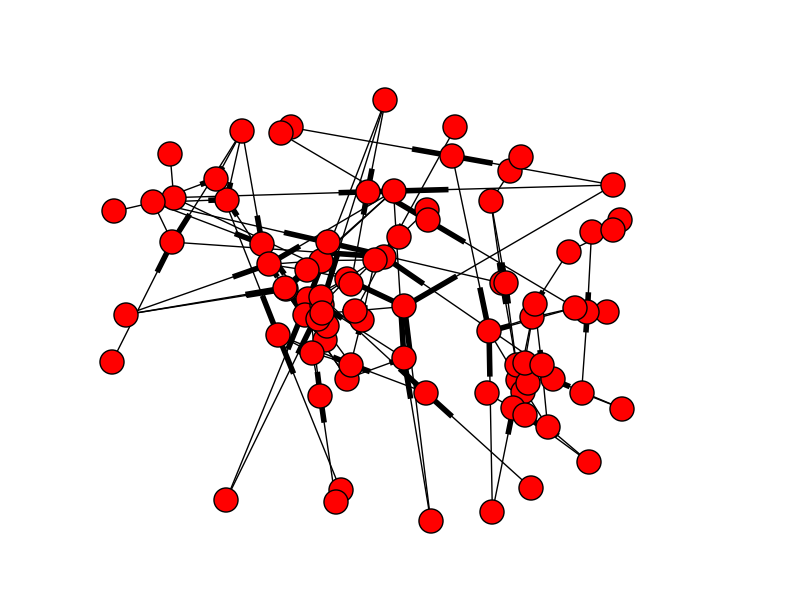
\includegraphics[scale=0.5]{network_stock_page_de_garde.png}\\
%----------------------------------------------------------------------------------------
%	AUTHOR SECTION
%----------------------------------------------------------------------------------------
\Large \emph{Authors:}\\
Antoine \textsc{Buffandeau}\\
Charles \textsc{François}\\
Mathieu \textsc{Gourmelen}\\
%\Large \emph{Supervisors:}\\
 \textsc{}
\\[1cm]
%----------------------------------------------------------------------------------------
%	DATE SECTION
%----------------------------------------------------------------------------------------
{\large \today} % Date, change the \today to a set date if you want to be precise
\vfill
\end{titlepage}
%----------------------------------------------------------------------------------------
%	INTRODUCTION SECTION
%----------------------------------------------------------------------------------------
\hypertarget{sec:part1}{}
\section{Introduction}
This report explores the structure of a stock correlation network created from a dataset of stock relationships. The dataset provides pairwise correlations between stocks, which are used to construct a network with connections based on specific correlation thresholds (0.3, 0.5, and 0.7). By applying network science techniques, the study investigates connectivity, community structures, core-periphery roles, and compares with two reference models: Erdős–Rényi and Barabási–Albert.
\begin{figure}[h!]
  \centering
  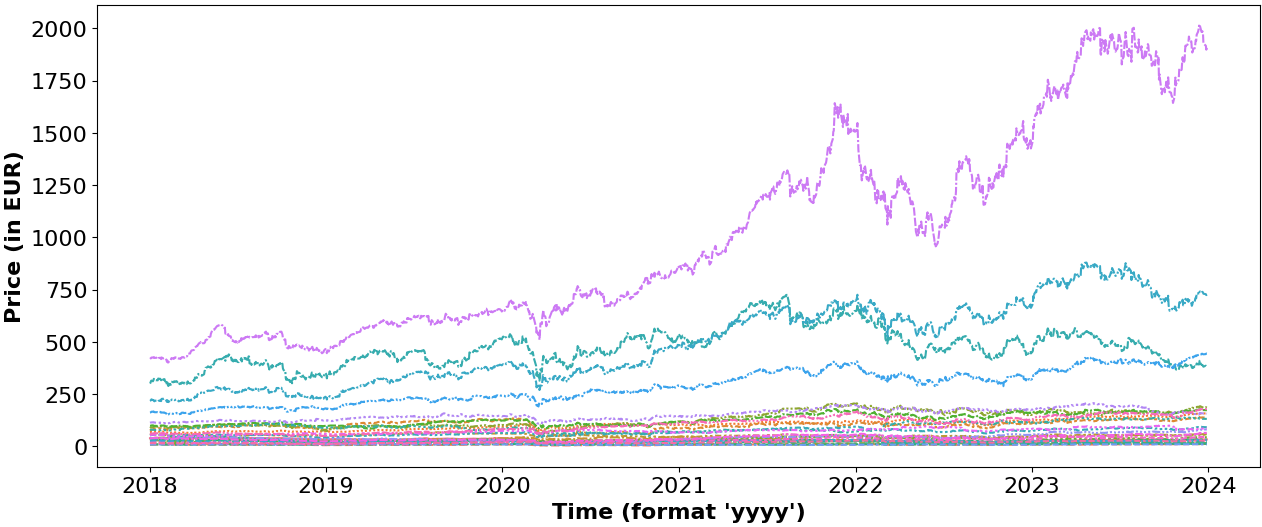
\includegraphics[width=\textwidth]{close_price_index_cac40_stocks.png}
  \caption{Daily closing prices of CAC 40 index stocks}
  \label{fig:stock_close_price}
\end{figure}
%----------------------------------------------------------------------------------------
%	TABLE OF CONTENTS SECTION
%----------------------------------------------------------------------------------------
\tableofcontents
\clearpage
%----------------------------------------------------------------------------------------
%	SECTION 1 
%----------------------------------------------------------------------------------------
\section{Dataset and Threshold-Based Network Construction}
The stock dataset contains correlation values between stock pairs, where each correlation reflects the strength of their relationship. Three networks were created based on thresholds (0.3, 0.5, and 0.7). These thresholds filter the connections, with lower thresholds allowing weaker correlations and resulting in denser networks, while higher thresholds retain only strong correlations, yielding sparser networks.
\begin{figure}[h!]
  \centering
  \begin{minipage}[b]{0.32\textwidth}
      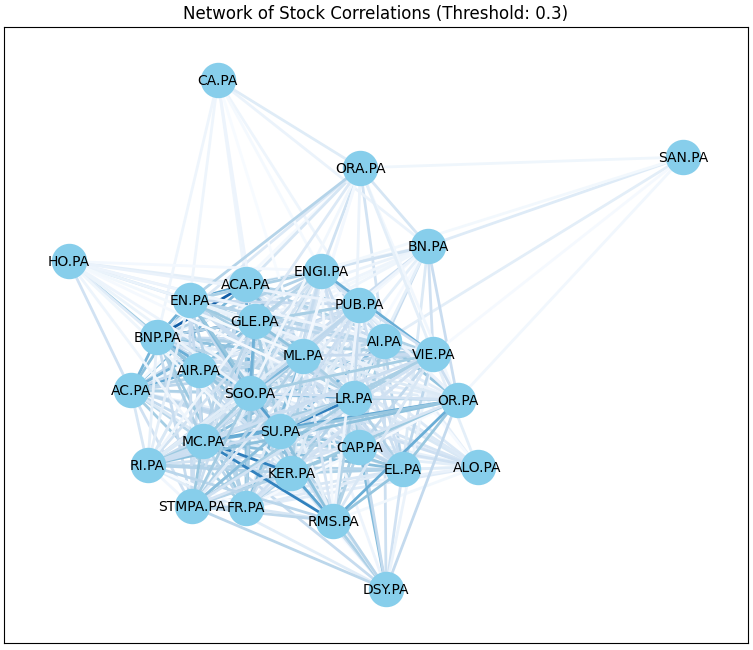
\includegraphics[width=\textwidth]{2D_network_stock_corr3.png}
      \caption{Threshold 0.3}
      \label{fig:threshold03}
  \end{minipage}
  \hfill
  \begin{minipage}[b]{0.32\textwidth}
      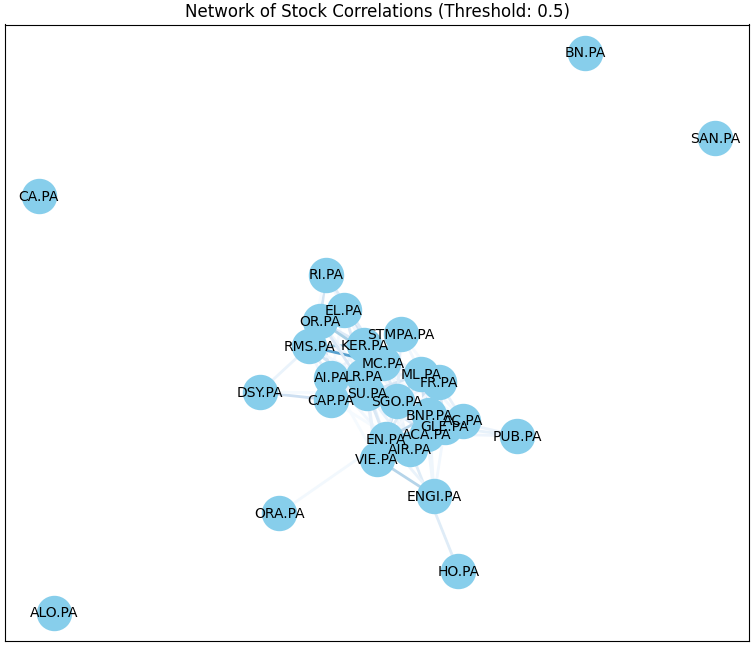
\includegraphics[width=\textwidth]{2D_network_stock_corr5.png}
      \caption{Threshold 0.5}
      \label{fig:threshold05}
  \end{minipage}
  \hfill
  \begin{minipage}[b]{0.32\textwidth}
      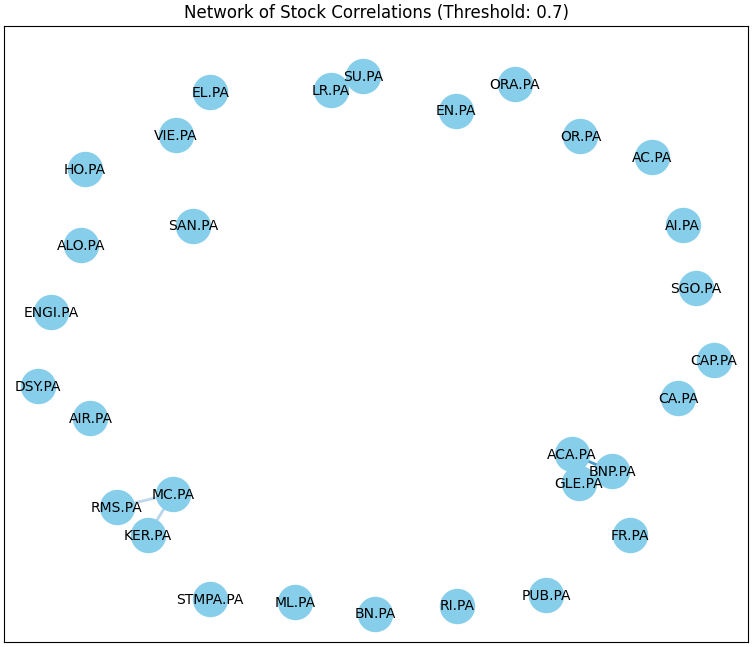
\includegraphics[width=\textwidth]{2D_network_stock_corr7.png}
      \caption{Threshold 0.7}
      \label{fig:threshold07}
  \end{minipage}
  %\caption{Network of Stock Correlations at Different Thresholds}
  \label{fig:stock_networks}
\end{figure}

\section{Step-by-Step Analysis}

\subsection{Step 1: Network Metrics}
Key metrics including average degree, density, transitivity, and assortativity were calculated for each thresholded network:
\begin{itemize}
    \item \textbf{Average Degree} decreases with increasing thresholds, indicating fewer connections as weaker correlations are removed.
    \item \textbf{Density} drops significantly from 0.8092 at 0.3 to 0.0138 at 0.7, confirming that the network becomes sparser.
    \item \textbf{Transitivity} shows high clustering at lower thresholds, remaining elevated at 0.3 but diminishing at 0.5 and 0.7.
    \item \textbf{Assortativity} is negative at lower thresholds, indicating a hub-like structure, and turns positive at 0.7, suggesting that remaining connections form among degree-similar nodes.
\end{itemize}

\begin{table}[H]
    \centering
    \begin{tabular}{|c|c|c|c|c|}
        \hline
        Threshold & Avg Degree & Density & Transitivity & Assortativity \\
        \hline
        0.3 & 23.47 & 0.8092 & 0.8957 & -0.1183 \\
        0.5 & 8.73 & 0.3011 & 0.6573 & -0.1053 \\
        0.7 & 0.4 & 0.0138 & 0.7500 & 0.2500 \\
        \hline
    \end{tabular}
    \caption{Network Metrics at Different Thresholds.}
\end{table}

\subsection{Step 2: Centrality Measures}
Four centrality metrics (degree, closeness, betweenness, eigenvector centrality) were calculated to identify influential stocks within each network. The results show that centrality is concentrated in fewer nodes at higher thresholds, indicating that only highly correlated stocks remain central in sparser networks.

\subsection{Step 3: Comparison with Network Models}
The constructed stock networks were compared to Erdős–Rényi and Barabási–Albert models:
\begin{itemize}
    \item \textbf{Erdős–Rényi Model} displayed low clustering and random connections, lacking the structural properties of the stock network.
    \item \textbf{Barabási–Albert Model} created a hub structure, forming a few highly connected nodes. While closer to the stock network, it did not fully capture the clustering observed in the data.
\end{itemize}

\begin{table}[H]
    \centering
    \begin{tabular}{|c|c|c|c|}
        \hline
        Model & Threshold & Transitivity & Assortativity \\
        \hline
        Stock Network & 0.3 & 0.8957 & -0.1183 \\
        Erdős–Rényi & 0.3 & 0.7970 & -0.0899 \\
        Barabási–Albert & 0.3 & 0.5488 & -0.3182 \\
        Stock Network & 0.7 & 0.7500 & 0.2500 \\
        Erdős–Rényi & 0.7 & 0.0000 & -0.5000 \\
        Barabási–Albert & 0.7 & 0.0000 & -0.3443 \\
        \hline
    \end{tabular}
    \caption{Comparison of Network Transitivity and Assortativity.}
\end{table}

\subsection{Step 4: Community Detection (Louvain Method)}
The Louvain method was applied to detect communities within each thresholded network. At lower thresholds, stocks naturally formed larger, densely connected communities, likely reflecting sector-based groupings or interrelated stocks. Modularity, which measures the strength of community division, was highest at threshold 0.3, indicating well-defined clusters.

\subsection{Step 5: Core-Periphery Analysis}
Using k-core decomposition, core-periphery structure was analyzed for each threshold:
\begin{itemize}
    \item \textbf{Core Stocks}: At threshold 0.3, multiple stocks formed the core, indicating strong interconnectedness within the network.
    \item \textbf{Periphery Stocks}: At threshold 0.7, only a small core remained, with most stocks in the periphery, showing a distinct separation between central and isolated stocks.
\end{itemize}

\section{Conclusion}
This network analysis reveals that the stock network differs significantly from random and scale-free models, exhibiting unique clustering, centrality, and core-periphery structures. As thresholds increase, connectivity decreases, isolating clusters of highly correlated stocks and leaving only a few central nodes. The results highlight the stock network’s natural clustering and centrality patterns, which suggest inherent relationships that might align with sectors or market dynamics.
%----------------------------------------------------------------------------------------
%	PART REFERENCES
%---------------------------------------------------------------------------------------
%\part{Références}
%\cite{EBA_website}
%\bibliographystyle{IEEEtran}
%\bibliography{ref_RS.bib}
%----------------------------------------------------------------------------------------
%	ENDING SECTION
%----------------------------------------------------------------------------------------
\end{document}